\documentclass[journal]{IEEE/IEEEtran}
\usepackage{pkg/pgf-pie}
\usepackage[T1]{fontenc}
\usepackage{inconsolata}
\usepackage{graphicx}

\graphicspath{ {images/} }

\usepackage{color}

\definecolor{pblue}{rgb}{0.13,0.13,1}
\definecolor{pgreen}{rgb}{0,0.5,0}
\definecolor{pred}{rgb}{0.9,0,0}
\definecolor{pgrey}{rgb}{0.46,0.45,0.48}
\usepackage{cite,graphicx,pgfplots,amsmath}
\usepackage{listings}
\lstset{language=Java,
  showspaces=false,
  showtabs=false,
  breaklines=true,
  showstringspaces=false,
  breakatwhitespace=true,
  commentstyle=\color{pgreen},
  keywordstyle=\color{pblue},
  stringstyle=\color{pred},
  basicstyle=\ttfamily,
%  moredelim=[il][\textcolor{pgrey}]{$$},
  moredelim=[is][\textcolor{pgrey}]{\%\%}{\%\%}
}



\newcommand{\SPTITLE}{UPLB Network Queue Simulator (UNQS): Surveying Network Performance Under Different Queueing Techniques For Internet Bandwidth Management}
\newcommand{\ADVISEE}{Leensey M. Lawas}
\newcommand{\ADVISER}{Danilo J. Mercado}

\newcommand{\BSCS}{Bachelor of Science in Computer Science}
\newcommand{\ICS}{Institute of Computer Science}
\newcommand{\UPLB}{University of the Philippines Los Ba\~{n}os}
\newcommand{\REMARK}{\thanks{Presented to the Faculty of the \ICS, \UPLB\
                             in partial fulfillment of the requirements
                             for the Degree of \BSCS}}
        
\markboth{CMSC 200 Undergraduate Thesis, \ICS}{}
\title{\SPTITLE}
\author{\ADVISEE~and~\ADVISER%
\REMARK
}
\pubid{\copyright~2016~ICS \UPLB}

%%%%%%%%%%%%%%%%%%%%%%%%%%%%%%%%%%%%%%%%%%%%%%%%%%%%%%%%%%%%%%%%%%%%%%%%%%

\begin{document}

% TITLE
\maketitle

% ABSTRACT
\begin{abstract}
Given the increasing demand for bandwidth, UNQS was developed to survey and to identify which among three queueing disciplines, namely, First In-First Out (FIFO), Priority Queue (PQ), and Weighted Fair Queueing (WFQ), produced the best performance as measured by duration (seconds), throughput (bits per second), and packet loss (percentage). The results show that while the simplest, FIFO showed the  best performance with minimal duration, maximal throughput, and minimal packet loss.
\end{abstract}

% INDEX TERMS
\begin{keywords}
bandwidth management, internet, network performance, network simulation, queueing, traffic engineering
\end{keywords}

% INTRODUCTION
\section{Introduction}
With the prevalence of internet usage in this digital age, the rise of demand for fast and reliable execution of online services is inevitable. Whether it is for personal use, like video chatting with friends and family from abroad, or for commercial and business transactions, customers want to make sure their services are done efficiently without slowing down or timing out. Client requests are sent simultaneously that when the server responses (or traffic) are returned, the routers are unable to inspect long fields in Internet Protocol (IP) packet headers quickly and are unable to reassemble and segment packets fast enough, causing performance bottleneck \cite{pazos_gerla_rigolio_1999}. A quick solution to the problem would be increasing bandwidth size, because as the demand for services increases, the bandwidth must also be increased \cite{communication_news_2001}. However, this method is costly and inefficient, which is why traffic engineering (TE) takes place. 

Awduche, Chiu, Elwalid, Widjaja, and Xiao of The Internet Society (2002) \cite{awduche_chiu_elwalid_xiao_2002} defined that internet traffic engineering deals with evaluating network performance and optimizing it. Bandwidth is the unit of measurement, usually in Kbps or Mbps, used to monitor network performance for quantifying how much information a communication channel can handle \cite{teach_ict_nd}.

\subsection{Background of the study}
Tong and Yang (2007)\cite{tong_yang_2007} cited that there have been many studies on TE, but most of them dealt with route selection algorithms, and few tackled bandwidth management techniques. For this study, bandwidth management is the TE method chosen. Kanu, Kuyoro, Ogunlere, \& Adegbenjo \cite{kanu_kuyoro_ogunlere_adegbenjo_2012} define bandwidth management as an optimization technique that helps differentiate the types of network traffic from each other and determine which client or service should be prioritized. In short, bandwidth management allocates the available bandwidth depending on network traffic and client/service priority.

In an article named \textit{Bandwidth management pays off} (2002)\cite{communication_news_2001}, two key devices were identified to help in bandwidth management: traffic shaping or congestion avoidance mechanisms and queueing techniques. \textit{Congestion avoidance mechanisms} or \textit{congestion control} locates where in the router the packets do not enter the system, and finds an alternative route so the packets do not block the way and cause timeout \cite{jacobson_1988}. \textit{Queueing techniques}, on the other hand, help predict and direct the traffic flow by implementing a constraint or constraints to provide the services as demanded \cite{gross_harris_1974}). In addition, queueing network models are known for accuracy and efficiency \cite{lazowska_zahorjan_graham_sevcik_1984}.

\subsection{Significance of the study}
Inefficient internet bandwidth management can lead to dissatisfied customers and reduced productivity. There have been many studies conducted to improve bandwidth management, but this study made use of queueing techniques to provide a simple yet novel and effective solution for managing internet bandwidth, particularly for the University of the Philippines Los Banos (UPLB) Network. While there is no imminent need to make use of a scheduling algorithm beside the traditional First Come-First Serve (FCFS) or First In-First Out (FIFO), it is undeniable that an increase of traffic coming in and out of the network will be expected. The results of this study can be helpful to determine if applying a different queueing scheduling algorithm will improve traffic flow at a given buffer size.

As long there will be a need for “high quality of corporate customer satisfaction”, bandwidth management will continue to grow as a body of knowledge \cite{duzbeck_2006}. That being said, this study aims to add to that body of knowledge by surveying three queueing scheduling algorithms and their effectivity as buffers for the traffic which will be passed from client to server and vice versa. Specifically, this study will monitor the UPLB Network traffic and simulate the traffic \clearpage using three queueing scheduling algorithms. By having this simulation, the advisable settings for the network will be identified, which in turn would provide effective bandwidth management.

\subsection{Objectives of the study}
The general objective of the study is to efficiently simulate the UPLB network traffic by identifying the most effective queueing technique. Specifically, the study should be able to:

\begin{enumerate}
\item Collect traffic data from the UPLB network;
\item Simulate the traffic data using the three queueing techniques;
\item Take note of the duration, throughput, and packet loss for each simulation; and
\item Determine the most effective queueing technique using graphs and simple statistics.
\end{enumerate}

\subsection{Time and Place of the study}
The study was conducted from January 2017 until May 2017, at the Institute of Computer Science, UPLB.

\subsection{Scope and Limitation of the study}
The study is limited to monitoring and simulating UPLB network. Also, it only made use of three queueing techniques, namely, First In-First Out Queueing (FIFO), Priority Queueing (PQ), and Weighted Fair Queueing (WFQ) or Priority Queuieng with aging.

In determining the most effective queueing technique, the throughput, latency, and packet loss values will be measured, noted, and compared. \textit{Throughput} is the number of tasks accomplished over a period of timem \textit{latency} is the time it takes for a fixed task to be finished \cite{martin_roth_nd}, and \textit{packet loss} is the percentage of dropped packets over the total number of packets.

The study shall be limited to monitoring and modeling the UPLB network.

\section{Review of Related Literature}
Several studies have been conducted which attempted to manage internet bandwidth as efficiently as possible. With a goal to provide speedy transaction of certain services such as e-mailing, video streaming, downloading, and many more, internet bandwidth management plays an important role not just for business and commerce applications, but as well as personal usage, for customer satisfaction and improved network performance. Because of the many details enumerated, the demand for internet bandwidth management has never been greater.

Internet users from 2015 to 2016 had increased with an estimated 43.4\% of the world population to 46.1\% \cite{internet_live_stats_2016}. It has been a dramatic increase since 1995, with users all over the world amounting less than 1\%. The implications of this statistics to the UPLB academe can also be applicable, as more students and workers enter the university to make use of the campus network. The increase entails a growth in demand for larger internet bandwidth. With a number of users sending multiple requests for different services with varying sizes, data traffic becomes congested. No end-user wants delays, slow downs, or timeouts, in accomplishing the services they requested. Instead, end-users want fast execution of their requests so they can proceed to doing other tasks.

To fix the problem, bandwidth management takes place. Instead of paying for an increase in bandwidth for a temporary fix \cite{communication_news_2001}, bandwidth management aims to properly allocate the already existing bandwidth size as effectively and as efficiently as possible.

Before packets are received by the destination address, they first arrive in packet switches. These packet switches are in charge of queueing the packets and forwarding them eventually to the destination \cite{comer_1999}. Thus enters the scheduling algorithms used to identify which packets must be distrbuted first to the computers in the network.

Traffic classification is an initial stage that plays a key role to the scheduling algorithms, particularly for the PQ and WFQ algorithms. Because of bandwidth contraints, traffic classification helps in managing the fixed, limited, and available bandwidth. Classification can be payload-based, meaning a field of the payload is examined and used for classification \cite[Chapter~5]{cisco_2008}. An early traffic classification technique \cite{schneider_1996} made use of port numbers, which worked best for well-known or reserved ports. The other method for classifcation uses statistical analysis of traffica behavior \cite[Chapter~5]{cisco_2008}.

A proposed priority packet scheduling algorithm \cite{karim_2012} made use of three priority queues that gave importance to real-time traffic (priority 1) over non-real time traffic (priorities 2 and 3). Its result suggested of a better performance opposed to FCFS and multi-level queue scheduler algorithms.

From a different study, packet scheduling algorithms using fair queueing and two additional variants were simulated to compare the delay. It showed that WFQ and Self Clock Fair Queueing (SCFQ) experienced a linear delay, whereas the Worst Case Weighted Fair Queueing (WF2Q) share the output link \cite{muhilan_2013}.

The aforementioned studies inspired and influenced this study, which shall use traffic data classified by protocol as input for the simulations of FIFO, PQ, and WFQ scheduling algorithms.

% MATERIALS AND METHODS
\section{Methodology}
\subsection{Traffic Collection}
With assistance from ITC, a mirror port was setup and connected to a 64-bit Ubuntu server named as \texttt{babage}. The traffic monitoring application, \texttt{ntopng}, was installed to the server. \texttt{MySQL} database management system was also installed, which shall contain the database where traffic flow data from \texttt{ntong} will be dumped. To run \texttt{ntopng}, a configuration file needs to be set to identify the network interface(s) and network(s) to be monitored, the database and table to be dumped at, and the HTTP port where the web portal can be accessed. Data was collected on April 17-18, 25, 28-29, and using the \texttt{mysqldump} tool, the .sql file was generated, which was used for the researcher to have a copy of the database outside of the UPLB network. 

\texttt{ntopng} uses ticks to measure the arrival of packets into the switch and their exit from switch to their destination. There are 66 million ticks per second \cite{webopedia_2017}, which means 1 tick is equal to 0.000000015 seconds. This value in seconds was multiplied to the tick value that \texttt{ntopng} collected.

\subsection{Simulation}
\subsubsection{Classes and their attributes}
\begin{enumerate}
\item \textbf{Cofiguration.java} - This class is responsible for setting, updating, validating, and displaying the configuration for the database connection (datestamp \textit{MM-DD-YY} and interface number \textit{i} for table name written as \textit{flows-MM-DD-YYv4\_i}, database name, IP address \textit{xxx.xxx.xxx.xxx}, password, port number \textit{p}, database username, database password) and queue settings (bandwidth \textit{b}, maximum buffer size \textit{m}, Maximum Transmition Unit \textit{mtu\_size}, queue type \textit{qt}.

\item \textbf{IPProtocol.java} - This class contains static variables to identify the protocols used for categorizing the priority of each packet into three queues. High priority queue have Transmission Control Protocol (TCP) and User Datagram Protocol (UDP) packets. Low priority packets use the following protocols: Internet Control Message Protocol (ICMP) and Host Identity Protocol. Internet Group Message Protocol (IGMP) and other protocols are classified into the normal queue.

\item \textbf{Main.java} - This contains the main function where the connection to database is established, and where time is looped starting from the minimum \texttt{FIRST\_SWITCHED} value (taken from the selected table and measured in ticks) until all packets are scheduled from packet switch to their destination.

\item \textbf{Packet.java} - A packet instance contains the following attributes: id, priority, protocol, size (in bytes), arrival time and send time to and from the scheduler (measured in ticks), and virtual time \textit{vt} (used only for WFQ).  Virtual time is computed as
\[
    vt = \frac{s}{w}
\]
where \textit{s} is the packet size and \textit{w} is the weight of a queue. Queue weight's value is derived as
\[
	w = d \times m
\]

where \textit{d} is the fixed distribution rate for each priority (0.5, 0.3, and 0.2 for high, medium, and low priorities respectively), and \textit{m} is the maximum buffer size.

\item \textbf{Queue.java} - Queue takes note of the current buffer size, packet count, total bytes transmitted, and maximum buffer size.

\item \textbf{Schedule.java} - Schedule has static-defined variables \textit{FIFO} (0), \textit{PQ} (1), and \textit{WFQ} (2). Its attributes are the schedule number and the total number of bytes transmitted.
\end{enumerate}

\subsubsection{Code snippet of the queue processing}
The code snippet in Figure \ref{fig:snippet} shows how the queues are being processed depending on the configured queue type. This method is called on per every iteration of time \textit{t}. The loop will stop once all the packets in the queues have been serviced.
\begin{figure}
\begin{lstlisting}

public boolean process(LinkedList<Queue> queues){
boolean success = false;

// process in order of arrival
if(schedule==Schedule.FIFO){
	Queue q = queues.remove();
	if(q.isEmpty()) return true;
	success = q.process(schedule);
	queues.add(0, q);
	return success;
}

// process from highest to lowest priority
else if(schedule == Schedule.PQ){
	for(int i=2; i>=0; i--){
	if(!queues.get(i).isEmpty()){
		Queue q = queues.remove(i);
		success = q.process(schedule);
		queues.add(i, q);
		return success;
 	}}
}

// process the smallest virtual time
else if(schedule == Schedule.WFQ){
	int pri = 0,
		smallest_virtual_time = 2147483647;
	Queue q;

	for(int i=2; i>=0; i--){
		q = queues.remove(i);
		if(!q.isEmpty()){					
		if( q.isEmpty() ) continue;
		else if(q.peek().virtual_time 
		< smallest_virtual_time){
		smallest_virtual_time = q.peek().virtual_time;
		pri = i;
		}}
		queues.add(i, q);
	}
	q = queues.remove(pri);
	success = q.process(schedule);
	queues.add(pri, q);
}

return success;	// true = nothing was processed or queue is empty. false = queue is not empty
}
\end{lstlisting}
\label{fig:snippet}\caption{Code Snippet of \textit{process} method in \texttt{Schedule.java}}
\end{figure}


\section{Results and Discussion}

\subsection{Description of Data per day}

\subsubsection{\textbf{April 17, 2017}}
The data collected on the first day spanned 28,823 ticks, garnering a total of 31,259 flows.

The top 3 source ports are as follows: port 0 with 4448 flows, port 5353 with 2247 flows, and port 137 with 1097 flows. Meanwhile, the top 3 destination ports are port 1900 (8528 flows), port 8000 (6153 flows), and port 0 (4448 flows).

The top 3 source IP addresses were 10.0.53.67 (4399 flows), 10.0.3.110 (3769 flows), and a tie for 10.0.53.53 and 10.0.3.148 (1764 flows). As for the destination IP addresses, 239.255.255.250 (9523), 10.0.3.53 (6174), and 224.0.0.252 (4088) ranked highest among other IP addresses.

\subsubsection{\textbf{April 18, 2017}}
For the second day, the data collection process took a total of 14,392 ticks, and recorded 20,574 flows.

The 3 most used source ports are ports 0, 5353, and 137, which were found in 2372, 1237, and 655 flows respectively. On the other hand, the top 3 frequented destination ports are noted to be port 8000 with 5439 flows, port 1900 with 5048 flows, and port 5355 with 2523 flows.

The 3 highest talkers for the day were IP addresses 10.0.53.53 (5444 flows), 10.0.3.110 (1825 flows), and 10.0.3.160 (1052 flows). Looking over to the receiving end, the top three destination IP addresses were 239.255.255.250 (5748 flows), 10.0.3.53 (5451), and 224.0.0.252 (3068).

\subsubsection{\textbf{April 25, 2017}}
The third day when the data was collected had a duration of 2498 ticks and a total of 3,892 flows, both of which are the shortest time span and smallest count of flows for the entire data set.

The top 3 source ports were port 0 (433), port 5353 (281), and port 138 (134). Destination ports most actively used were ports 8000 (1344 flows), 1900 (890), and 0 (433).

Hosts that sent most packets through the network came from IP addresses 10.0.53.177 (1359), 10.0.3.110 (319), and 10.0.3.89 (168). Three IP addresses that received the most requests that day were 10.0.3.53 (1359), 239.255.255.250 (991), and 224.0.0.252 (365).

\subsubsection{\textbf{April 28, 2017}}

Data gathered for the fourth day lasted for a length of 11,812 ticks and observed a total of 11,483 flows in the network.

Ports that were used to send out the most interaction are ports 0 (2220), 5353 (897), and 138 (532). Ports that received the most interaction are ports 1900 (3789), 0 (2220), and 5355 (1473).

The most active source IP address is 10.0.3.110 (1529), followed by 10.0.3.148 (817), and 10.0.3.89 (689). On the other hand, the most active destination IP addresses are 239.255.255.250 (4312), 224.0.0.252 (1959), and 224.0.0.251 (1423).


\subsubsection{\textbf{April 29, 2017}}

The fifth and final data collection counted 14,027 flows within a time frame of 7183 ticks.

Topping as a source port is port 0 with 1197 flows, followed by port 5353 at 600 flows, and lastly, port 138 with 281 flows. The three highest ranking destination ports are as follows: port 8000 counted 7924 flows; port 1900 had 2253; and port 0 registered 1197 flows.

Three source nodes most notably active were of IP addresses 10.0.53.9 (7967), 10.0.3.110 (932), and 10.0.3.148 (369). On the receiving end, the following are the top 3 IP addresses: 10.0.3.53 (7970), 239.255.255.250 (2525), and 224.0.0.251 (861).
\linebreak
\hrule

In summary, the observed frequented applications being used can be seen by the ports used most. Port 8000 is used by the Hyper Text Transfer Protocol, port 1900 is used by the Simple Service Discovery Protocol, port 0 is the initial 'binding' port before the operating system returns a new value, which is an available port, and port 5355 is used for Link-Local Multicast Name Resolution.

\subsection{Metrics Considered in the Data Analysis}
The following figures show bar graphs of the average network performance metrics to be looked at: duration, throughput, and packet loss. The dates per collection, from left to right, are April 17, 18, 25, 28, and 29. The data that spawned these results were collected 4 hours per date. For each scheduling algorithm, ten varying buffer sizes were tested, from 10MB, 20MB...until 100MB. The averages for each network performance metric were collected and visualized in the figures.

\subsubsection{Duration}

\begin{figure}
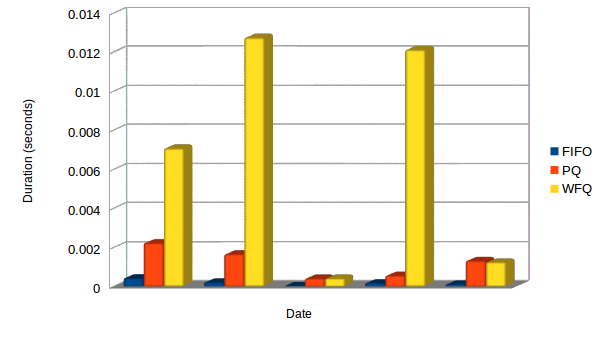
\includegraphics[width=0.5\textwidth]{duration}
\label{fig:duration}\caption{Average Durations per Date and Queue Type}
\end{figure}

It is evident from \ref{fig:duration} that in terms of how fast the packets are scheduled, \texttt{WFQ} takes the most time to finish in scheduling the packets. Duration \textit{d} is a function of the arrival time \textit{t\textsubscript{0}} and last switched time \textit{t\textsubscript{n}} seen as follows:

\[
	d(t_0, t_n) = t_n - t_0
\]

\subsubsection{Throughput}
\begin{figure}
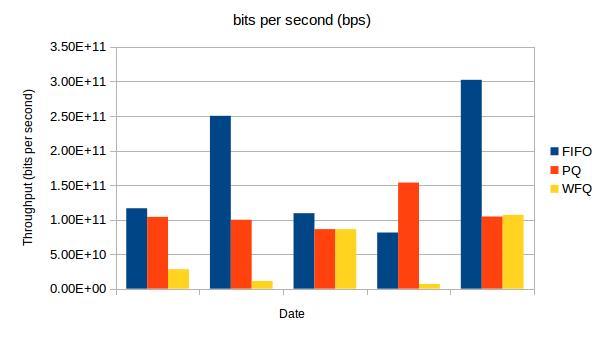
\includegraphics[width=0.5\textwidth]{throughput}
\label{fig:throughput}\caption{Average Throughputs per Date and Queue Type}
\end{figure}

Throughput \textit{tput} was computed as 
\[
	tput = \frac{count(p_s)}{d}
\]

where \textit{ts} is the total size (in bytes) that was successfully switched, and \textit{d} as the computed duration. Focusing on \ref{fig:throughput}, \texttt{FIFO} scheduling queue outputted the most throughput.

\subsubsection{Packet Loss}
\begin{figure}
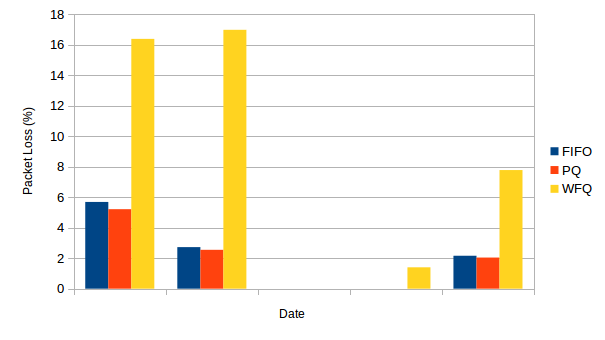
\includegraphics[width=0.5\textwidth]{packetloss}
\label{fig:packetloss}\caption{Average Packet Losses per Date and Queue Type}
\end{figure}

The last network performance parametric looked at is the packet loss \textit{l}, solved by

\[
	l = \frac{count(p_l)}{count(p_l + p_s)} \times 100
\]

where all dropped packets \textit{p\textsubscript{l}} are counted, divided by the total of dropped \textit{p\textsubscript{l}} and switched packets \textit{p\textsubscript{s}} multiplied by 100, to get the percentage. Similarly, the results show that \texttt{WFQ} has the worst performance when packet loss is considered. Notably, \texttt{PQ} shows lower packet loss compared to \texttt{FIFO}.

\subsubsection{Bandwidth Constraint}
In attempt to check if the same trend is observed when a bandwidth constraint is added, the following bandwidth constraints were tested using a 100MBps buffer: 600Mbps, 800Mbps, 1000Mbps, and 1200Mbps. These values were converted into their byte form and with help from the conversion value for seconds to ticks, they were translated into 1.125 Bytes per tick (Bpt), 1.5Bpt, 1.875Bpt, and 2.25Bpt respectively. The result is visualized in \ref{fig:bc}. The throughputs noted for all ran simulations are very close to the bandwidth, and a 100MB buffer provided 0\% packet loss, hence only the duration was left as  basis.

As seen, PQ and WFQ amounted to the same duration that showed improvement per increase of the bandwidth. Yet, it is apparent that FIFO's performance is a lot better based on this network performance metric. FIFO, in any of the bandwidth constraints, displayed minimal and fast speed of switching the packets, while maintaining a similar throughput to the slow-performing PQ and WFQ.

\begin{figure}
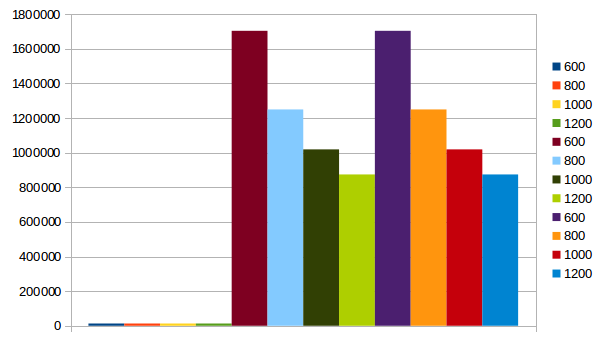
\includegraphics[width=0.5\textwidth]{duration_with_bc}
\label{fig:bc}\caption{Average Durations with Applied Bandwidth Constraint}
\end{figure}

\section{Conclusion and Recommendation}
After the experiment, the results show that the UPLB network works better using the \texttt{FIFO} scheduling algorithm. It was able to output the most number of packets over a period of time, as shown by \ref{fig:throughput}, and switched the packets fastly \ref{fig:duration} while maintaining the most integrity by minimizing lost packets\ref{fig:packetloss}.

While \texttt{PQ} and \texttt{WFQ} algorithms were intended to improve the network performance in terms of packet switching, this study proves that the traffic of UPLB is more suited to a \texttt{FIFO} scheduling algorithm.

For future studies, the researcher would recommend that a different traffic classification method is to be used, such as statistical methods or machine learning methods. Another advisable method is to inspect a different field of the payload or packet that will be used to classify traffic, instead of the protocol field. A final recommendation is the use of hybrid or variation of the PQ and WFQ scheduling algorithms to further improve the switching, thus effectively managing UPLB's internet bandwidth.

% BIBLIOGRAPHY
\bibliographystyle{./IEEE/IEEEtran}
\bibliography{./cs190-ieee}
% \nocite{*}

% BIOGRAPHY
\begin{biography}[{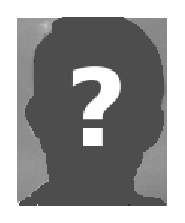
\includegraphics{./yourPicture.eps}}]{\ADVISEE}
She is a BS Computer Science undergraduate student. She not only writes code, but also songs, poems, and stories.
\end{biography}

\end{document}
